% \chapter{Trabajo}

% Preface
% \note{Soy un estudiante italiano en Erasmus. Hablo español bastante bien, pero me resulta más natural escribir en inglés; sin embargo, decidí escribir en español para practicar, con la ayuda de algunos traductores cuando era necesario. Si hay algo mal escrito o poco claro, estoy a disposición para cualquier aclaración.}

\chapter{Trabajo académico - Planificación Inteligente}

\lstset{language=python}



\note{Soy un estudiante italiano en Erasmus. Hablo español bastante bien, pero me resulta más natural escribir en inglés; sé que un compañero prenguntó si podía escribir en inglés, y que está bien. sin embargo, decidí escribir en español para practicar, con la ayuda de algunos traductores cuando era necesario. Si hay algo mal escrito o poco claro, estoy a disposición para cualquier aclaración.}

\section{Introducción}

{He eligido el \textbf{dominio de emergencias} para mi trabajo. Resumiendo lo que está escrito en la tarea, en este dominio los puntos de interés son los siguientes:\ns
\begin{itemize}
   \item Localización de las víctimas, ambulancias y hospitales.
   \item Asignación de ambulancias a las víctimas, teniendo en cuenta la gravedad de la emergencia.
   \item Traer a todas las víctimas a un hospital, como objetivo.
\end{itemize}}

La version más basica del escenario incluye una sola víctima, en vez la version ampliada mas victímas.

\framedt{Definición Problema}{

   Para implementar una solucción al problema de la planificación de emergencias con \textsc{pyhop}, es útil formalizar el problema en términos de:
   \begin{itemize}
      \item \textbf{Estado inicial}: la localización de las víctimas, ambulancias y hospitales.
      \item \textbf{Estado objetivo}: las víctimas han sido trasladadas a los hospitales.
      \item \textbf{Dominio} (acciones disponibles): mover ambulancias, cargar y descargar
      víctimas, tratar a las víctimas en las ambulancias.
   \end{itemize}
   
   \begin{itemize}
      \item \textbf{Sujetos estáticos}: localizaciones y hospitales.
      \item \textbf{Sujetos dinámicos}: ambulancias y víctimas.
   \end{itemize}
   
   \vspace{0.5em}
}

\section{Implementación}

\subsection{Organización del código}
{El código se divide en tres ficheros:\ns
\begin{itemize}
   \item \texttt{emerg.py}: contiene la implementación de las funciones de los operadores y métodos.
   \item \texttt{scenario.py}: contiene la definición de posibles estado iniciales.
   \item \texttt{utils.py}: contiene funciones auxiliares, para trazar el grafico de la ciudad de Valencia y imprimir algunos mensajes.
\end{itemize}}
Para ejecutar el código se puede usar el comando \texttt{python3 emerg.py}, añadiendo el parámetro \texttt{-A} se generan animaciones de los movimientos de las ambulancias en un fichero \texttt{.mp4}.
Si lo prefiere puede utilizar \textsc{Docker}, para evitar la instalación de las dependencias necesarias.

\begin{verbatim}
   docker build -t emergencia .
   docker run -v $(pwd)/output:/app/output -e PARAMS="-A" emergencia
   docker run -v $(pwd)/output:/app/output emergencia    # without animations
\end{verbatim}



\subsection{Representación del estado}
El estado se representa con alguno diccionarios, uno para cada entidad:
\begin{lstlisting}
   state1.ambulances = [ {'label': 'A1', 'cap': 10, 'loc': 'El Carmen'},...
   state1.victims = [ {'name': 'Carlos', 'sev': 5, 'loc': 'El Carmen'},...
   state1.hospitals = [ {'name': 'H1', 'loc': 'Hospital La Fe'},...
   state1.coordinates = { 'El Carmen': {'x': 50, 'y': 50}, 'Ciutat Vella': {'x': 55, 'y': 45}, ...
\end{lstlisting}
En cada entrada de cada diccionario se encuentran propiedades de la entidad como la posición, el nombre y la gravedad.

Las localidades son barrios/areas de la ciudad de Valencia, y cada barrio es caracterizado por coordenadas \lstinline|(X,Y)|.
Se asume que es posible viajar entre cualquier par de localizaciones y el tiempo de viaje es proporcional a la distancia euclídea entre ambas.
\begin{figure}[htbp]
   \centering
   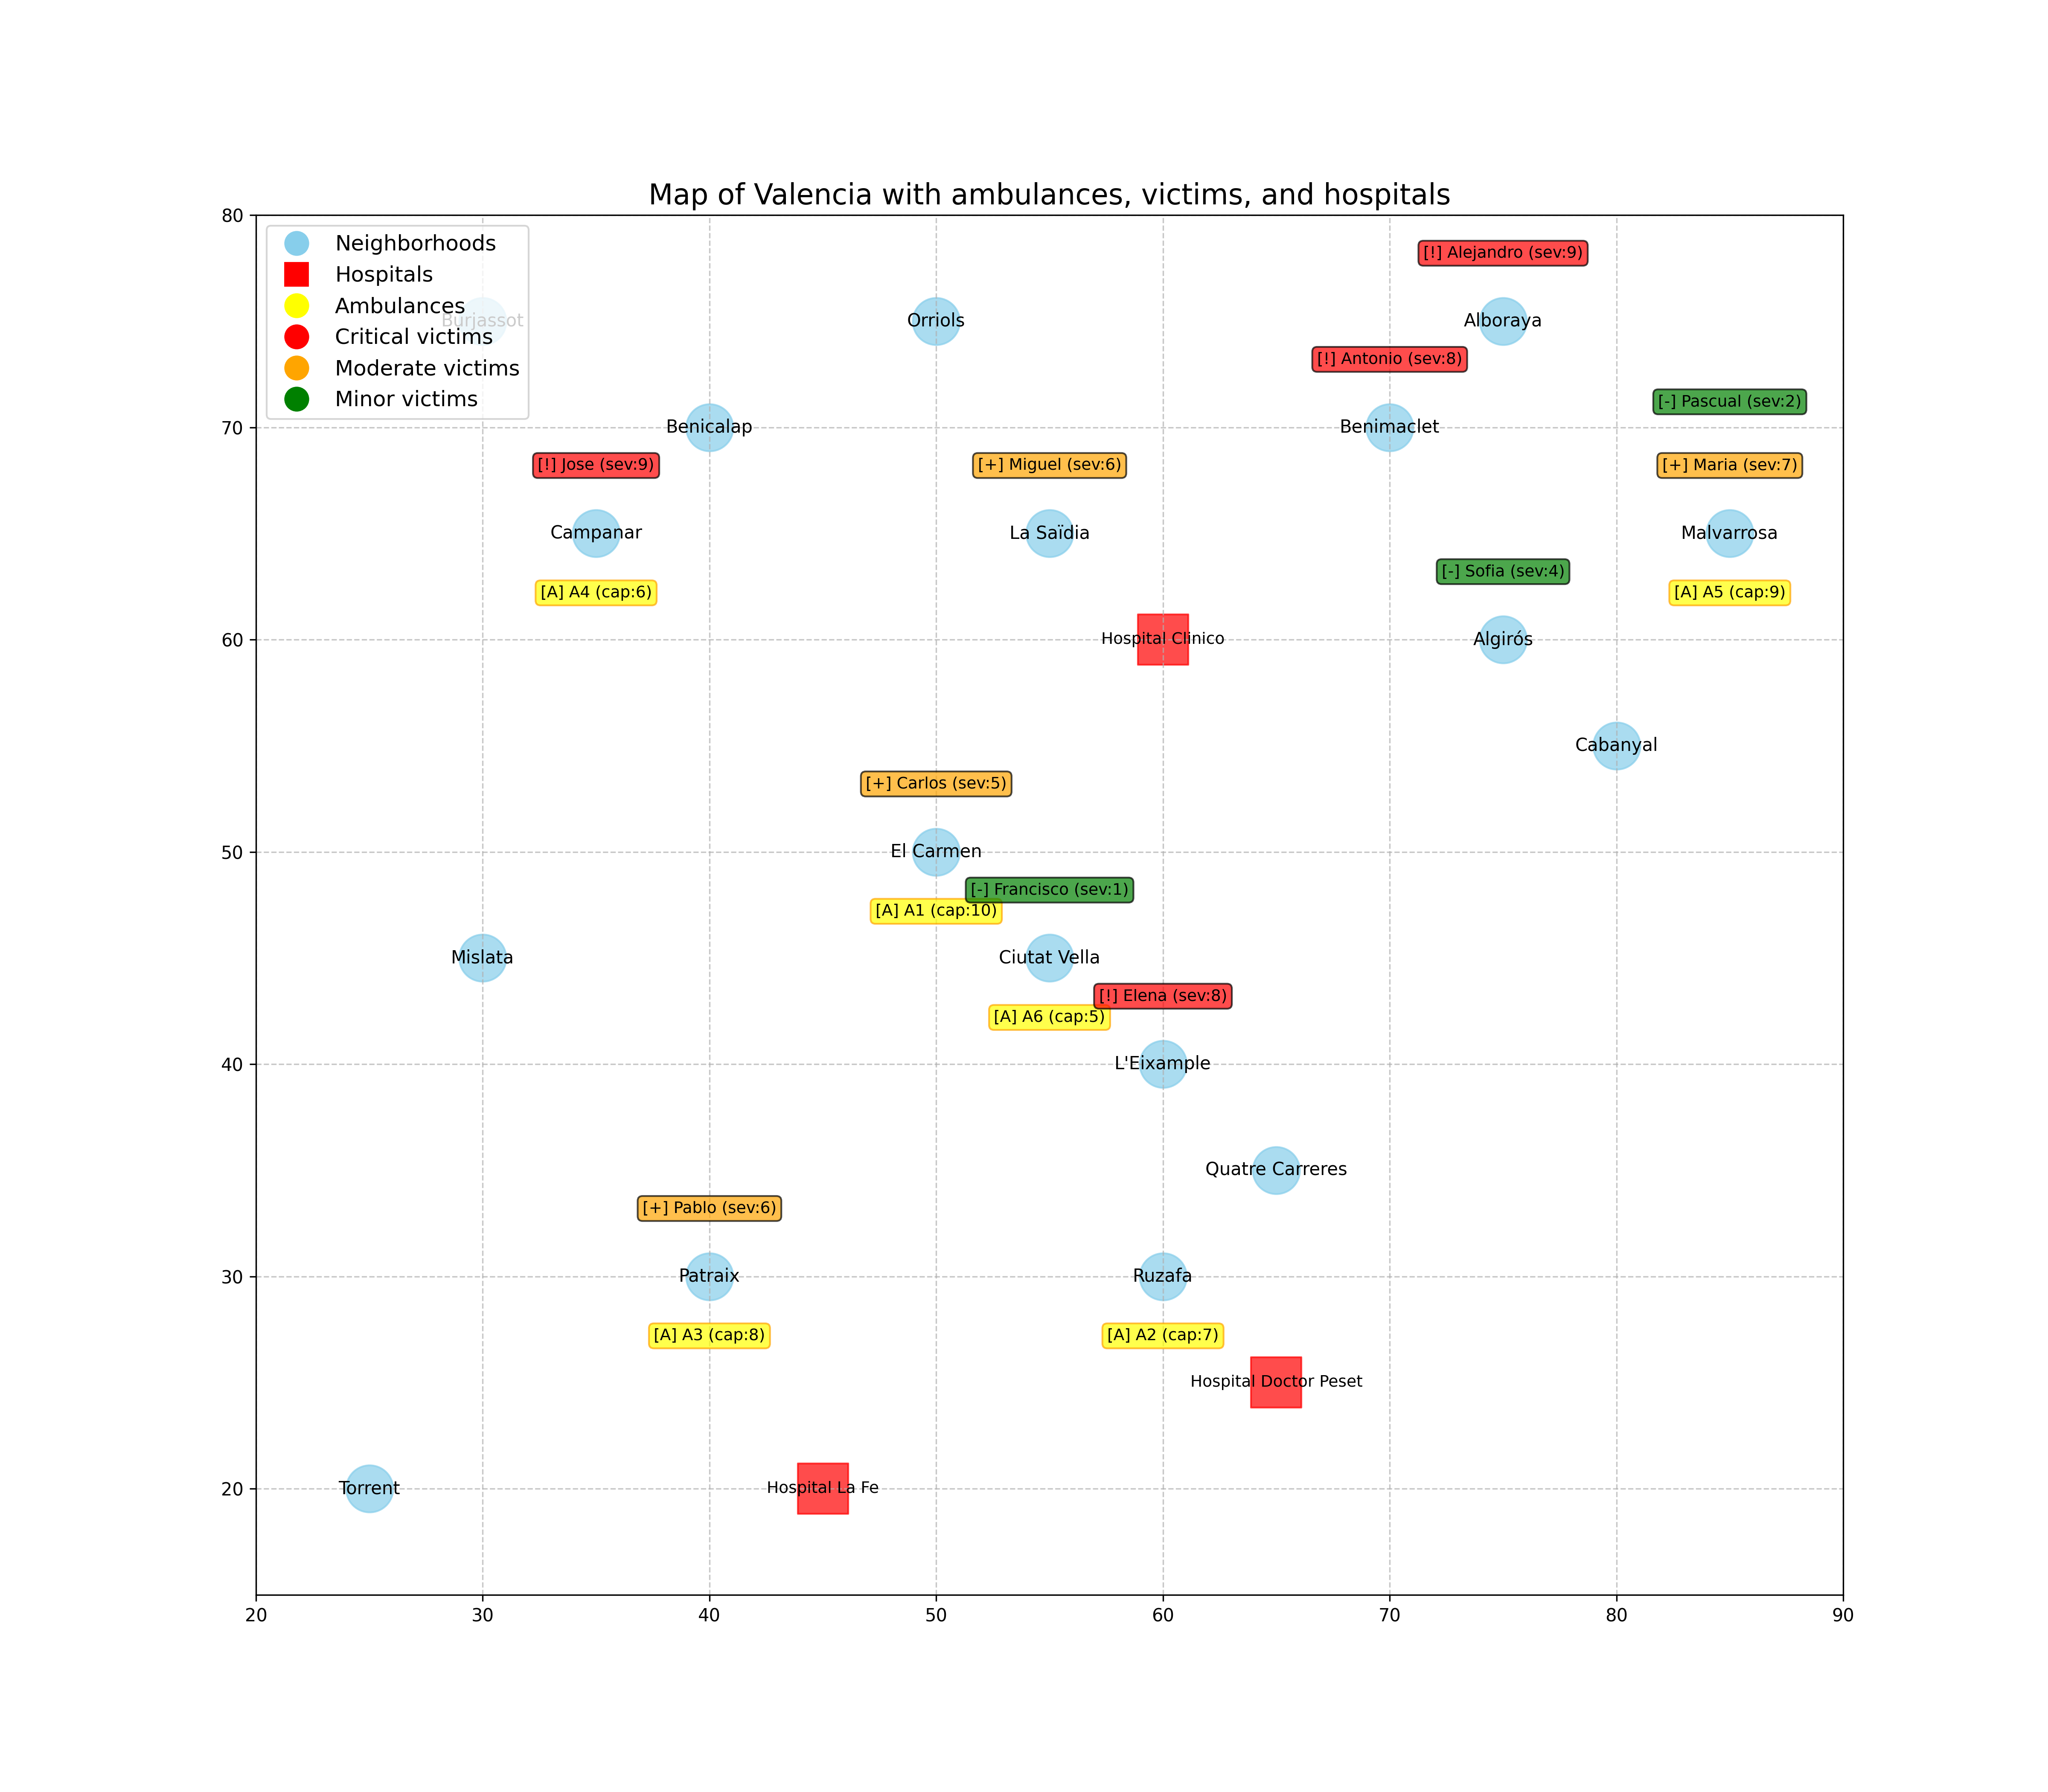
\includegraphics{images/valencia_map.png}
   \caption{Barrios de Valencia}
   \label{fig:valencia_map}
\end{figure}

\subsection{Operadores}

Los \textit{operadores} de \textsc{pyhop} representan las acciones que se pueden realizar en el dominio, y no so se pueden descomponerse. Se devuelve al nueve estado tras aplicarse el operador o \lstinline|False| si el operador falla (i.e. no se aplicable).
Entonces los operadores en nuestro dominio son lo siguientes, que son bastante self-explanatory:
\begin{itemize}
   \item \lstinline|op_drive(state, amb, dest)| - Mover la ambulancia a una localización. Puede parecer complicado pero es solo porque hay algunas instrucciones para trazar el camino en el mapa, que no es necesario para la planificación, pero es útil para la visualización. 
   \item \lstinline|op_load(state, amb, victim)| - Cargar una víctima en una ambulancia. Aquí tenemos que verificar que la ambulancia tiene suficiente capacidad para la severidad de la víctima.
   La localización de la víctima se convierte en la propia ambulancia que la traslada.
   \note{Nel código esto control se hace también en el método \lstinline|method_deliver_victim|.}
   \item \lstinline|op_unload(state, amb, victim, hospital)| - Descargar una víctima en un hospital.
   \item \lstinline|op_treat(state, amb, victim)| - Tratar a una víctima en una ambulancia si su gravedad supera el umbral de la primera asistencia.
   \item \lstinline|op_remove_victim(state, victim_name)| - Solo remueve la víctima de la lista de víctimas.
\end{itemize}

\subsection{Métodos}

Los \textit{métodos} implementan la logica de la planificación, y determinan la secuencia de operadores que se deben aplicar para alcanzar un objetivo.

El método fundamental es \lstinline|method_deliver_victim(state, victim_dict, hospital)|, que se utiliza para mover la ambulancia más cercana a la víctima, cargar la víctima, mover la ambulancia al hospital y descargar la víctima.
Este método es lo más sencillo, y es invocado por los otros métodos para resolver el problema de las víctimas múltiples.


La manera más intuitiva y sencilla de implementar la gestión de multiple victímas es de llamar recursivamente el método de búsqueda para cada victima, escribiendo algo así:
\begin{lstlisting}[caption={Esto no se encuentra en el codigo entregado}, captionpos=b]
   def method_deliver_all(state):
   if not state.victims:
       return []  # Base case: no more victims to deliver.
   
       # Take the first victim in the list.
       victim = state.victims[0]
       return [('deliver_victim', victim, 'H1'),
           ('op_remove_victim', victim['name']),
           ('deliver_all',)]
\end{lstlisting}

Sin embargo, el orden en que se entregan las víctimas afecta a la travel distance, porque el estado de las ambulancias cambia después de cada entrega, entonces, la solucción óptima no es la misma que la solucción de los subproblemas.\\
Parece claro que el orden en que se entregan las víctimas afecta a la travel distance;
las instrucciones del trabajo no piden específicamente tratar este tema, de hecho, concierne a la optimización, no a la planificación, para la cual es simplemente importante alcanzar el estado final, pero me intrigó y pensé que merecía la pena analizarlo.

He implementado cuatro métodos para entregar todas las víctimas, que vamos a describir más detalladamente abajo en la Sec. \ref{sec:ordenar_victimas}.
\begin{itemize}
   \item \lstinline|method_deliver_all_severity_priority(state)| - Entregar todas las víctimas en orden de severidad.
   \item \lstinline|method_deliver_all_distance_priority(state)| - Entregar todas las víctimas en orden de distancia a la ambulancia más cercana.
   \item \lstinline|method_deliver_in_order(state)| - Entregar las víctimas simplemente en el orden en que se encuentran en la lista.
   \item \lstinline|method_try_all_permutations(state, max_victims=5)| - Probar todas las permutaciones de las víctimas y devolver la que minimiza la distancia total recorrida y la que minimiza el \textit{makespan}.\\
   El código de este método parece complicado da leer, pero en realidad es bastante simple, solo tiene que manejar algunas variables de tracking para controlar las permutaciones y las distancias.
   \note{Hay un umbral \lstinline|max_victims| para limitar el número de permutaciones que se prueban, porque el número de permutaciones crece muy rápidamente con el número de víctimas. Sobre el umbral se generan solo \lstinline|max_victims!| permutaciones, y se eligen casualmente.}
\end{itemize}

\section{Observaciones}

\subsection{Ordenar víctimas}
\label{sec:ordenar_victimas}

Antes de decidir como ordinar las victímas es necesario definir un criterio de optimización. He considerado tres posibles funciones objetivo:
\begin{enumerate}
   \item \textbf{Severidad} de emergencia - Prioritizar las víctimas más graves: esto es ---más o menos--- lo que se prefiere hacer en un escenario real, sin embargo, no conduce a minimizar la distancia de viaje\footnote{Puede ocurrir, pero por casualidad.}.
   Esta función objetivo es la más fácil de implementar, porque se puede ordenar la lista de víctimas por severidad y luego entregarlas en ese orden, no hay muchas decisiones que tomar, solo que la ambulancia más cercana a la víctima se mueve a su localización.
   \begin{lstlisting}
   def method_deliver_all_severity_priority(state):
      if not state.victims:
          return []  # Base case: no victims left
      # Sort victims by severity (most severe first)
      victims_by_severity = sorted(state.victims, key=lambda v: v['sev'], reverse=True)
      victim = victims_by_severity[0] # The most severe victim
      best_hosp = # The closest hospital
      return [('deliver_victim', victim, best_hosp['name']),
              ('method_deliver_all_severity_priority',)]
   \end{lstlisting}
   \newpage
   \item \textbf{Travel distance} - Minimizar la distancia total recorrida por las ambulancias. Para hacer esto he implementado un algoritmo \textit{greedy}, que elige primero la víctima que tiene la más cercana ambulancia. 
   \begin{lstlisting}
   def method_deliver_all_distance_priority(state):
      # ...
      for victim in state.victims:
         for amb in state.ambulances:
             if amb['cap'] >= victim['sev']:  # Ambulance can handle this victim
                 dist = euclidean_distance(amb['loc']),victim['loc'] ))
                 if dist < min_distance:
                     min_distance = dist
                     best_victim = victim
      # ...
   \end{lstlisting}

   No estaba seguro de si esto garantizaba la solución óptima, así que intenté enumerar todas las permutaciones de víctimas y calcular la distancia total para cada permutación, y parece ---salvo errores en la implementación ---que la solución greedy ya proporciona la distancia óptima.\\
   Para hacer esto hay el método \lstinline|method_try_all_permutations(state, max_victims=5)|, que prueba todas las permutaciones, y se puede observar como la mejor solucción que encuentra es la misma que la solucción greedy.
   \note{No he probado todas las permutaciones de ambulancias para cada victima en cada permutación, he utilizado como criterio de elección de la ambulancia lo mismo que en los otros métodos, la ambulancia más cercana a la victima.}
   \item \textbf{Makespan} - Asumiendo como dice el texto que el tiempo de viaje es proporcional a la distancia euclídea entre dos localizaciones, se puede considerar que dos ambulancias distintas pueden viajar \textbf{simultáneamente}, entonces, el tiempo total de respuesta es el tiempo que tarda la última ambulancia en llegar al hospital.\\
   Un buen algoritmo para minimizar el makespan puede ser de utilizar el mayor número posible de ambulancias, pero no he implementado este método. En vez, se observa que, como es lógico, en relación con el makespan, las permutaciones casuales generadas por \lstinline|method_try_all_permutations()| pueden ofrecer a menudo mejores resultados que el algoritmo greedy utilizado para minimizar \textit{travel distance}.
\end{enumerate}

\subsection{Estados iniciales}

En \texttt{scenario.py} se definen cuatro estados iniciales con distintas configuraciones de víctimas y ambulancias, para probar el código. Se puede elegir uno de ellos añadiendo la siguientes opciones al comando de ejecución:
\begin{enumerate}
   \item \texttt{-S1} - Una sola víctima
   \item \texttt{-S1} - 5 víctimas, donde todas las permutaciones de las víctimas son evaluadas.
   \item \texttt{-S1} - 5 víctimas, la planificación tiene que fallar porque no hay ninguna ambulancia capaz de transportar a la víctima más grave.
   \item \texttt{<Default>} - 11 víctimas, que no permite de evaluar todas la permutaciones, solo algunas eligidas casualmente, y en efecto observamos cómo distintas ejecuciones dan resultados diferentes.
\end{enumerate}



\subsection{Leer los resultados}

El código imprime los resultados en un formato verboso pero bastante linear.
Aquí hay un ejemplo de la salida para el escenario con 11 víctimas.
\note{Hay omisiones por razones de brevedad.}


En la primera sección, el se imprime el resultado del metodo 
\lstinline|method_deliver_all_distance_priority|, que minimiza la distancia total recorrida por las ambulancias, incluyendo el viaje de cada ambulancia e el makespan, aunque no sea el objetivo del método.
\lstset{inputencoding=utf8/latin1}
\begin{verbatim}
   --- DISTANCE PRIORITIZATION APPROACH ---
   
   --- FULL AMBULANCE MOVEMENT REPORT ---
   
   Ambulance A1 started at: El Carmen
     1. From El Carmen to El Carmen (empty) - distance: 0.00
     2. From El Carmen to Hospital Clinico (Carlos) - distance: 14.14
     3. From Hospital Clinico to La Saïdia (empty) - distance: 7.07
      ...
     9. From Hospital Clinico to L'Eixample (empty) - distance: 20.00
     10. From L'Eixample to Hospital Doctor Peset (Elena) - distance: 15.81
     Total distance for A1: 122.38
   
   Ambulance A3 started at: Patraix
     1. From Patraix to Patraix (empty) - distance: 0.00
     2. From Patraix to Hospital La Fe (Pablo) - distance: 11.18
     Total distance for A3: 11.18
   
   Ambulance A5 started at: Malvarrosa
     1. From Malvarrosa to Malvarrosa (empty) - distance: 0.00
     2. From Malvarrosa to Hospital Clinico (Maria) - distance: 25.50
      ...
     8. From Malvarrosa to Hospital Clinico (Pascual) - distance: 25.50
     Total distance for A5: 169.90
   
   Ambulance A6 started at: Ciutat Vella
     1. From Ciutat Vella to Ciutat Vella (empty) - distance: 0.00
     2. From Ciutat Vella to Hospital Clinico (Francisco) - distance: 15.81
     Total distance for A6: 15.81
   
   Verified total distance: 319.27
   Makespan (parallel time): 169.90 units (critical ambulance: A5)
   =====================================
\end{verbatim}

En la segunda sección se generan las permutaciones con el método \lstinline|method_try_all_permutations|, e imprime la distancia y el makespan uno de cada 10, e al final
el resultado de las 5 mejores permutaciones por distancia y por makespan, junto con la ambulancia que determina el makespan (la que ha hecho el viaje más largo).
\begin{verbatim}
   --- PERMUTATION OPTIMIZATION APPROACH ---
   Too many victims (11) to try all permutations.
   Sampling 120 random permutations from 39916800 possibilities...
   Tested permutation 10 starting with Pablo: distance 337.87, makespan 161.34 (A5)
   Tested 10/120 permutations. Best distance: 319.27
   Tested permutation 20 starting with Carlos: distance 337.70, makespan 260.75 (A5)
   Tested 20/120 permutations. Best distance: 319.27
   ...
   Tested permutation 120 starting with Francisco: distance 345.98, makespan 289.04 (A5)
   Tested 120/120 permutations. Best distance: 319.27
   
   ===== TOP 5 PERMUTATIONS BY TOTAL DISTANCE =====
   1. Order: ['Pascual', 'Pablo', ..., 'Sofia'] - Distance: 319.27 - Makespan: 171.62 (A5)
   ...
   5. Order: ['Maria', 'Alejandro', ..., 'Miguel'] - Distance: 319.27 - Makespan: 180.22 (A1)
   
   ===== TOP 5 PERMUTATIONS BY MAKESPAN =====
   1. Order: ['Miguel', 'Pascual',..., 'Maria'] - Makespan: 112.61 - Distance: 350.90 (A2)
   ...
   5. Order: ['Miguel', 'Pascual', ..., 'Antonio'] - Makespan: 147.20 - Distance: 350.90 (A5)
   Time taken: 0.47 seconds
   Makespan (parallel time): 112.61 units (critical ambulance: A2)
   =====================================
\end{verbatim}

Al final se imprime un resumen de los resultados, comparando los dos métodos, \lstinline|method_deliver_all_distance_priority| y \lstinline|method_try_all_permutations|, y se calcula el porcentaje de mejora de la travel distance y del makespan.

\begin{verbatim}
   --- COMPARISON ---
   TOTAL DISTANCE:
     Distance optimization: 319.27 units
     Victim order: ['Alejandro', 'Sofia', 'Antonio', 'Jose', 'Francisco', 'Carlos', 'Elena', 'Miguel', 'Pascual', 'Maria', 'Pablo']
     Permutation optimization: 319.27 units
     Victim order: ['Pascual', 'Pablo', 'Miguel', 'Carlos', 'Alejandro', 'Antonio', 'Elena', 'Maria', 'Jose', 'Francisco', 'Sofia']
     Improvement: 0.00%
   
   MAKESPAN (PARALLEL TIME):
     Distance optimization: 169.90 units, critical ambulance: A5
     Victim order: ['Alejandro', 'Sofia', ..., 'Pablo']
     Permutation optimization: 112.61 units, critical ambulance: A2
     Victim order: ['Miguel', 'Pascual', ..., 'Maria']
     Improvement: 33.72%
\end{verbatim}

\subsection{Animaciones}

El código genera una mapa del estado inicial en un fichero \texttt{valencia\_map.jpg}, que incluye localizaciones, ambulancias y víctimas.\\
Si se añade el parámetro \texttt{-A} al comando de ejecución, se generan animaciones de los movimientos de las ambulancias en dos ficheros \texttt{.mp4}.
Me resultaron muy útiles para tener una representación visual del plan ejecutado por \textsc{pyhop}.
\note{Tengo que admitir que no conozco muy bien la librería \texttt{matplotlib}, y que pedí a una IA generativa que me ayudara a escribir las funciones para renderizar el mapa y las animaciones. \smiley}


\section{Conclusiones}

\textsc{pyhop} permite de modelar y resolver problemas de planificación de manera sencilla y elegante, y es muy útil para problemas de planificación que se pueden descomponer en acciones elementales.\\
Hay maneras de resolver el problema sin formalizar los métodos de planificación, pero durante la realización de este trabajo, me he dado cuenta de que siguiendo el esquema de \textsc{pyhop} se obtiene un código más claro y legible, así como una representación linear del dominio.

El problema de la planificación de emergencias es un problema interesante y complejo, especialmente si se considera también como optimizar una solucción en términos de travel distance y makespan, en vez de limitarse a planificar para alcanzar un estado final; se puede complicar más si se van a consider multiplés funciones objetivo.
En un escenario real, la severidad de la emergencia es importante, pero no es el único factor a considerar, es necesario también minimizar el tiempo de respuesta para todas la víctimas.\\
En general, he leido online que el \textit{Emergency Vehicle Dispatching Problem} es una variante del \href{https://en.wikipedia.org/wiki/Vehicle_routing_problem}{\textit{Vehicle Routing Problem}} (VRP), que es un problema NP-hard, que pero parece diferir dal nuestro problema en algunos aspectos, sobre todo que en el VRP hay un grafo con arcos que tienen un costo asociado y que determinen entre cuales nodos se puede viajar, mientras en nuestro problema se puede viajar entre cualquier par de nodos. Podemos imaginar que el nuestro es un caso particular en que el grafo es completo.

Y además, en la realidad, no siempre todos los hospitales están disponibles, el tráfico afecta a la travel distance, y otros factores tecnicos (carburante, turnos de trabajo, mantenimiento de vehículos, \dots) y éticos/humanos pueden influir en la solucción elegida.

